\documentclass[ngerman]{gdb-aufgabenblatt}


\renewcommand{\Aufgabenblatt}{5}
\renewcommand{\Ausgabedatum}{Mi. 09.12.2015}
\renewcommand{\Abgabedatum}{Do. 08.01.2016}
\renewcommand{\Gruppe}{Kraemer, Mirzada, Frangopoulos, Heid}
\renewcommand{\STiNEGruppe}{06}
\renewcommand{\Semester}{WS 2015/16}


\begin{document}


\section*{Aufgabe 1: Referentielle Aktionen}
\subsection*{a) Anforderungen an sicheres Schema}
Das Ergebnis der referentiellen Aktionen darf nicht von der Reihenfolge der Ausf�hrung dieser abh�ngig sein.

\subsection*{b) Referenzgraph}
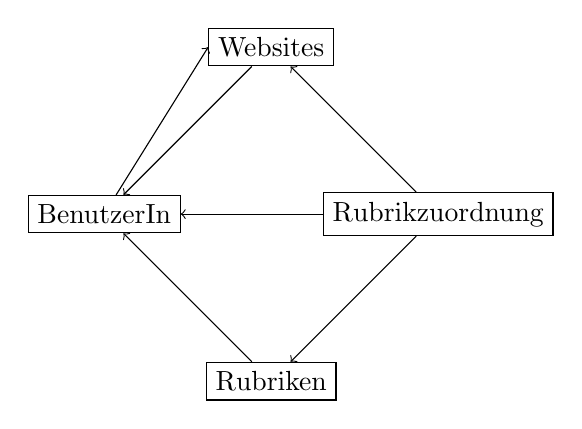
\begin{tikzpicture}[->, node distance=3cm]
\node[draw] (Websites) at (0,0) {Websites};
\node[draw] (BenutzerIn) [below left of= Websites] {BenutzerIn};
\node[draw] (Rubrikzuordnung) [below right of= Websites] {Rubrikzuordnung};
\node[draw] (Rubriken) [below right of= BenutzerIn] {Rubriken};

\draw[->] (Websites) 		-- (BenutzerIn);
\draw[->] (Rubrikzuordnung) -- (BenutzerIn);
\draw[->] (Rubriken) 		-- (BenutzerIn);
\draw[->] (BenutzerIn) 		-- (Websites.west);
\draw[->] (Rubrikzuordnung) -- (Websites);
\draw[->] (Rubrikzuordnung) -- (Rubriken);


\end{tikzpicture}

\subsection*{c) Unsicherheit}
Beim L�schen eines Eintrags aus BenutzerIn gibt es 2 unterschiedliche m�gliche Effekte auf die Eintr�ge von Rubrikzuordnung.\\
Das L�schen k�nnte auf direktem Weg kaskadieren oder per indirektem Weg �ber Rubriken verboten werden.

\subsection*{d) Vorkehrungen}
Referenz auf BenutzerIn von Rubrikzuordnung : On Delete CASCADE -> On Delete RESTRICT


\section*{�nderbarkeit von Sichten}

\begin{RMSchma}
Person(\soliduline{PID}, Name, Vorname, \dashuline{(HaustierName, HaustierRasse) $\rightarrow$ (Haustier.Name, Haustier.Rasse)})

Haustier(\soliduline{Name, Rasse}, \dashuline{Herrchen $\rightarrow$ Person.PID})
\end{RMSchma}






\section*{Serialisierbarkeit und Anomalien}
\subsection*{a) Belegungen}
\begin{tabular}{|c|c|c|c|c|c|c|}
\hline
&$S_1$&$S_2$&$S_3$&$S_4$&$S_5$&$S_6$\\
\hline
$A$&$305$&$195$&$300$&$190$&$115$&$300$\\
\hline
$B$&$195$&$5$&$5$&$5$&$5$&$5$\\
\hline
\end{tabular}
\subsection*{b) Abh�ngigkeiten}

\begin{tabular}{|c|l|}
\hline
$S_1$&Die Operation $r_2(A)$ ist abh�ngig von Operation $w_1(A)$.\\
\hline
$S_2$&Hier sind keine Operationen voneinander abh�ngig.\\
\hline
$S_3$&Die Operation $r_1(B)$ ist von der Operation $w_2(B)$ und die Operation $r_1(A)$ von der Operation $w_2(A)$ abh�ngig.\\
\hline
$S_4$&Die Operation $r_1(B)$ ist von der Operation $w_2(B)$ abh�ngig.\\
\hline
$S_5$&Hier sind keine Operationen voneinander abh�ngig.\\
\hline
$S_6$&Die Operation $r_1(B)$ ist von der Operation $w_2(B)$ und die Operation $r_1(A)$ von der Operation $w_2(A)$ abh�ngig.\\
\hline
\end{tabular}

\subsection*{c) Serialisierbarkeit}
\begin{tabular}{|c|l|}
\hline
$S_1$&Der Schedule ist seriell. $T_1$ wird vor $T_2$ ausgef�hrt.\\
\hline
$S_2$&Der Schedule ist nicht serialisierbar, da bei einer Nacheinanderausf�hrung der \\
&Transaktionen bestimmte Leseoperationen abh�ngig von vorher geschehenen\\
&Schreiboperationen w�ren. Dies ist bei $S_2$ nicht der Fall.\\
\hline
$S_3$&Der Schedule ist serialisierbar. Es wird nach der Serialisierung $T_2$ vor $T_1$ ausgef�hrt.\\
\hline
$S_4$&Der Schedule ist nicht serialisierbar.\\
\hline
$S_5$&Der Schedule ist nicht serialisierbar, da bei einer Nacheinanderausf�hrung der \\
&Transaktionen bestimmte Leseoperationen abh�ngig von vorher geschehenen \\
&Schreiboperationen w�ren. Dies ist bei $S_5$ nicht der Fall.\\
\hline
$S_6$&Der Schedule ist seriell. Es wird $T_2$ vor $T_1$ ausgef�hrt.\\
\hline
\end{tabular}

\newpage
\section{Aufgabe 4: Transaktionen}


\section{Beispiel f�r Operatorbaum}

\begin{tikzpicture}
\node (Haustier) {Haustier};
\node (Wolf) [left=25mm of Haustier] {Wolf};
\node (join1) [above=20mm of $(Haustier)!.5!(Wolf)$] {$\verbund{Wolf.WID=Haustier.HID}$};
\node (selektion1) [above=of join1] {$\selektion{Name=\wert{Hasso}}$};
\node (projektion) [above=of selektion1] {$\projektion{Rasse}$};
\node (final) [above=of projektion] {};

\path (Haustier) edge node[smallr,near start,above right] {?? Tupel\\?? Attribute} (join1);
\path (Wolf) edge node[smalll,near start,above left] {?? Tupel\\?? Attribute} (join1);
\path (join1) edge node[smallr,near start,above left] {?? Tupel\\?? Attribute} (selektion1);
\path (selektion1) edge node[smallr,midway,left] {$??\cdot\frac{??}{??}=??$ Tupel\\?? Attribute} (projektion);
\path (projektion) edge node[smallr,midway,left] {$??$ Tupel\\1 Attribut} (final);
\end{tikzpicture}







\section{Beispiel f�r Tabelle mit Sperranforderungen}

\begin{tabular}{|p{2cm}|p{2cm}|p{2cm}|p{2cm}|p{1cm}|p{1cm}|p{1cm}|p{3cm}|}
\hline
Zeitschritt & T\ts{1} & T\ts{2} & T\ts{3} & x & y & z & Bemerkung\\
\hline
\hline
0 &  &  &  & NL & NL & NL & \\
\hline
1 & lock(x,X) &  &  & X\ts{1} & NL & NL & \\
\hline
2 & write(x) & lock(y,R) &  & X\ts{1} & R\ts{2} & NL & \\
\hline
3 &  &  &  &  &  &  & \\
\hline
4 &  &  &  &  &  &  & \\
\hline
5 &  &  &  &  &  &  & \\
\hline
\end{tabular}



\section{*Thema*}

*L�sung*






\end{document}